\chapter{Экспериментальная оценка и анализ результатов}
\label{ch:experiments}

\section{Цель и принципы проведения экспериментов}

Экспериментальная часть работы предназначена для практической проверки пригодности разработанного программного комплекса к задачам системного анализа, а также для демонстрации того, каким образом получаемые измерения могут использоваться при сравнении реальных вычислительных платформ. В отличие от чисто теоретического обсуждения архитектуры приложения, данный раздел ориентирован на подтверждение того, что предложенный подход позволяет формировать интерпретируемые, устойчивые и прикладно значимые результаты в условиях реальных операционных систем и фоновой активности.

Цель экспериментальной части состоит не только в сравнении двух платформ различной архитектуры и программной среды, но и в проверке воспроизводимости измерений комплекса «Системный анализатор», а также в анализе того, насколько удобен разработанный инструмент для практической интерпретации результатов. Иными словами, в рамках экспериментов оценивается не только поведение тестируемого оборудования, но и состоятельность самого подхода, основанного на объединении телеметрии и синтетических бенчмарков в едином интерфейсе.

В качестве тестовых систем рассматриваются:
\begin{itemize}
    \item MacBook Air 15'' (M2, 2023), macOS Ventura+;
    \item ASUS Vivobook 15 (Ryzen 5 4600H), Windows 11.
\end{itemize}

Выбор именно таких платформ обусловлен их различием как по микроархитектуре, так и по программной среде. Одна система относится к семейству современных ARM-совместимых энергоэффективных платформ Apple Silicon, вторая --- к x86-64 платформам массового сегмента на базе мобильного процессора AMD Ryzen. Такое сопоставление представляет интерес не только с прикладной точки зрения, но и с методической: оно позволяет оценить, насколько разработанный комплекс способен корректно функционировать в неоднородных программно-аппаратных условиях и предоставлять сопоставимый формат результата при наличии различий в операционной системе, механизмах энергосбережения, драйверной модели и наборе доступных метрик.

При интерпретации результатов принципиально учитывается то обстоятельство, что измерения в многозадачной операционной системе неизбежно содержат шум. Любой запуск теста происходит не в изолированной лабораторной среде, а в системе, где параллельно работают фоновые службы, диспетчеры окон, сетевые стеки, файловые индексы и другие процессы. Для уменьшения влияния случайных факторов в комплексе используются разогрев, серия итераций и робастная статистическая обработка, включающая фильтрацию выбросов и оценку разброса результатов. Дополнительно в ходе эксперимента фиксируются условия выполнения: режим питания, наличие фоновой нагрузки, версия ОС и общая характеристика тестовой конфигурации.

С методической точки зрения эксперименты строятся на нескольких принципах. Во-первых, сравнение должно выполняться не по одному изолированному числу, а по совокупности результатов, характеризующих различные классы нагрузок. Во-вторых, любые числовые показатели должны интерпретироваться с учётом качества измерения и телеметрического контекста. В-третьих, выводы по экспериментальной части должны быть сформулированы не как абстрактное ранжирование платформ, а как анализ сильных и слабых сторон каждой системы применительно к конкретным профилям вычислительных задач.

\section{Методика и условия выполнения}

Корректность экспериментальной оценки в значительной степени зависит от единообразия условий выполнения тестов. Даже при использовании одного и того же программного комплекса результаты могут существенно различаться, если один прогон проводится при высокой фоновой нагрузке, а другой --- в близком к «чистому» состоянии системы. Поэтому методика эксперимента включает набор организационных требований, направленных на снижение влияния плохо контролируемых факторов.

Перед запуском измерений рекомендуется:
\begin{enumerate}
    \item закрыть ресурсоёмкие приложения и дождаться завершения фоновых задач (обновления, индексация);
    \item подключить устройство к сети питания (или, если цель — оценка «в полевых условиях», явно зафиксировать режим работы от батареи);
    \item зафиксировать параметры системы: модель CPU, объём RAM, объём и тип накопителя, версию ОС;
    \item выполнить по крайней мере 3 независимых прогона каждой категории, сравнивая медианные значения и коэффициент вариации.
\end{enumerate}

Каждый из перечисленных пунктов имеет практическое и методическое значение. Закрытие ресурсоёмких приложений уменьшает вероятность паразитной конкуренции за CPU, память и дисковую подсистему. Подключение к сети питания важно для исключения искажений, связанных с агрессивными профилями энергосбережения, особенно на ноутбуках. Фиксация конфигурации системы необходима для корректного документирования эксперимента и последующего воспроизведения условий. Наконец, выполнение нескольких независимых прогонов позволяет перейти от единичного наблюдения к статистически более осмысленной оценке.

Важным элементом методики является также предварительный анализ состояния системы перед началом каждой серии тестов. Пользователь или исследователь должен учитывать текущую загрузку ядер, наличие активных фоновых процессов, дисковую и сетевую активность, а также общее время работы системы после загрузки. Например, запуск бенчмарка сразу после включения компьютера может сопровождаться активностью служб инициализации, а проведение измерений после длительной работы под нагрузкой может приводить к иному тепловому режиму и, как следствие, к другим частотным характеристикам процессора.

В рамках дипломной работы результаты представляются в виде таблиц по основным категориям бенчмарков: «Процессор», «Память», «Математика», «Криптография». Отдельно приводятся скриншоты интерфейса комплекса, позволяющие зафиксировать форму представления данных и иллюстрировать, каким образом пользователь наблюдает состояние системы и результаты запусков. Наличие графических иллюстраций важно не только как элемент визуального сопровождения, но и как подтверждение того, что разработанный комплекс действительно обеспечивает единый контур наблюдения и измерения.

На рис.~\ref{fig:main_window} показан главный экран комплекса с набором вкладок, а на рис.~\ref{fig:memory_tests} --- пример панели тестов памяти, демонстрирующей формат отображения результатов и единицы измерения.

\begin{figure}[!htbp]
\centering
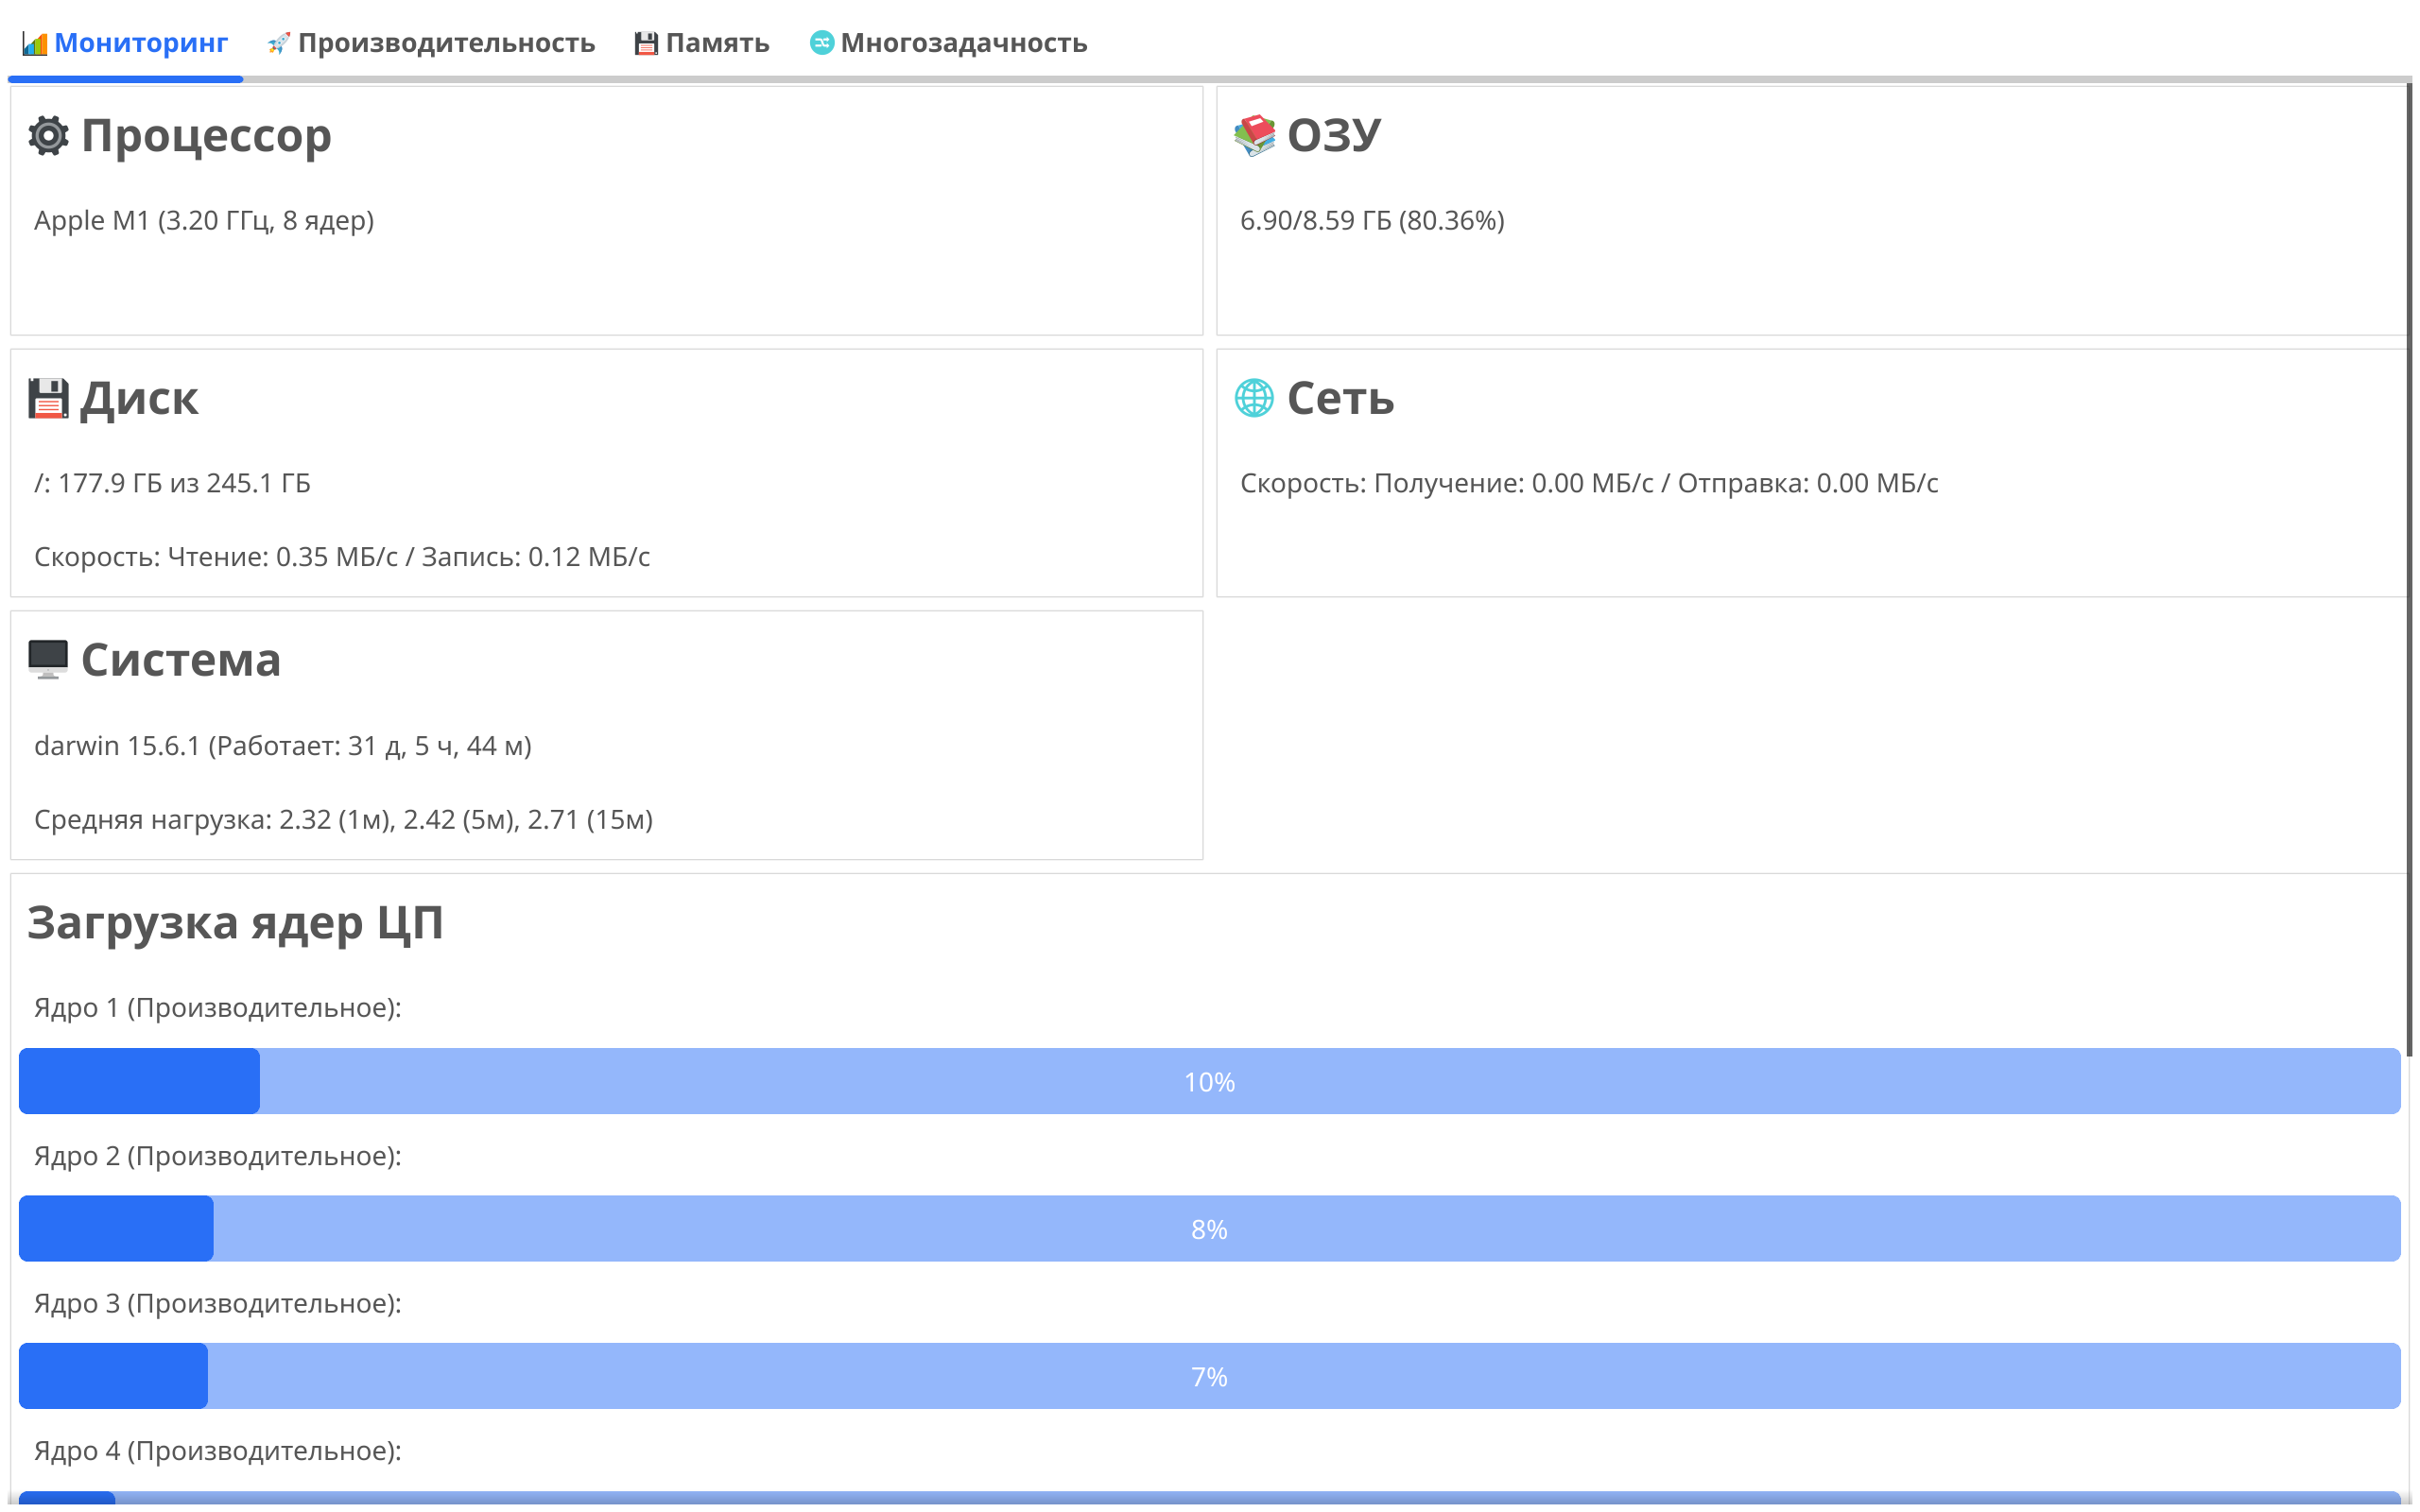
\includegraphics[width=0.92\textwidth]{main_window.png}
\caption{Главное окно комплекса «Системный анализатор»}
\label{fig:main_window}
\end{figure}

\begin{figure}[!htbp]
\centering
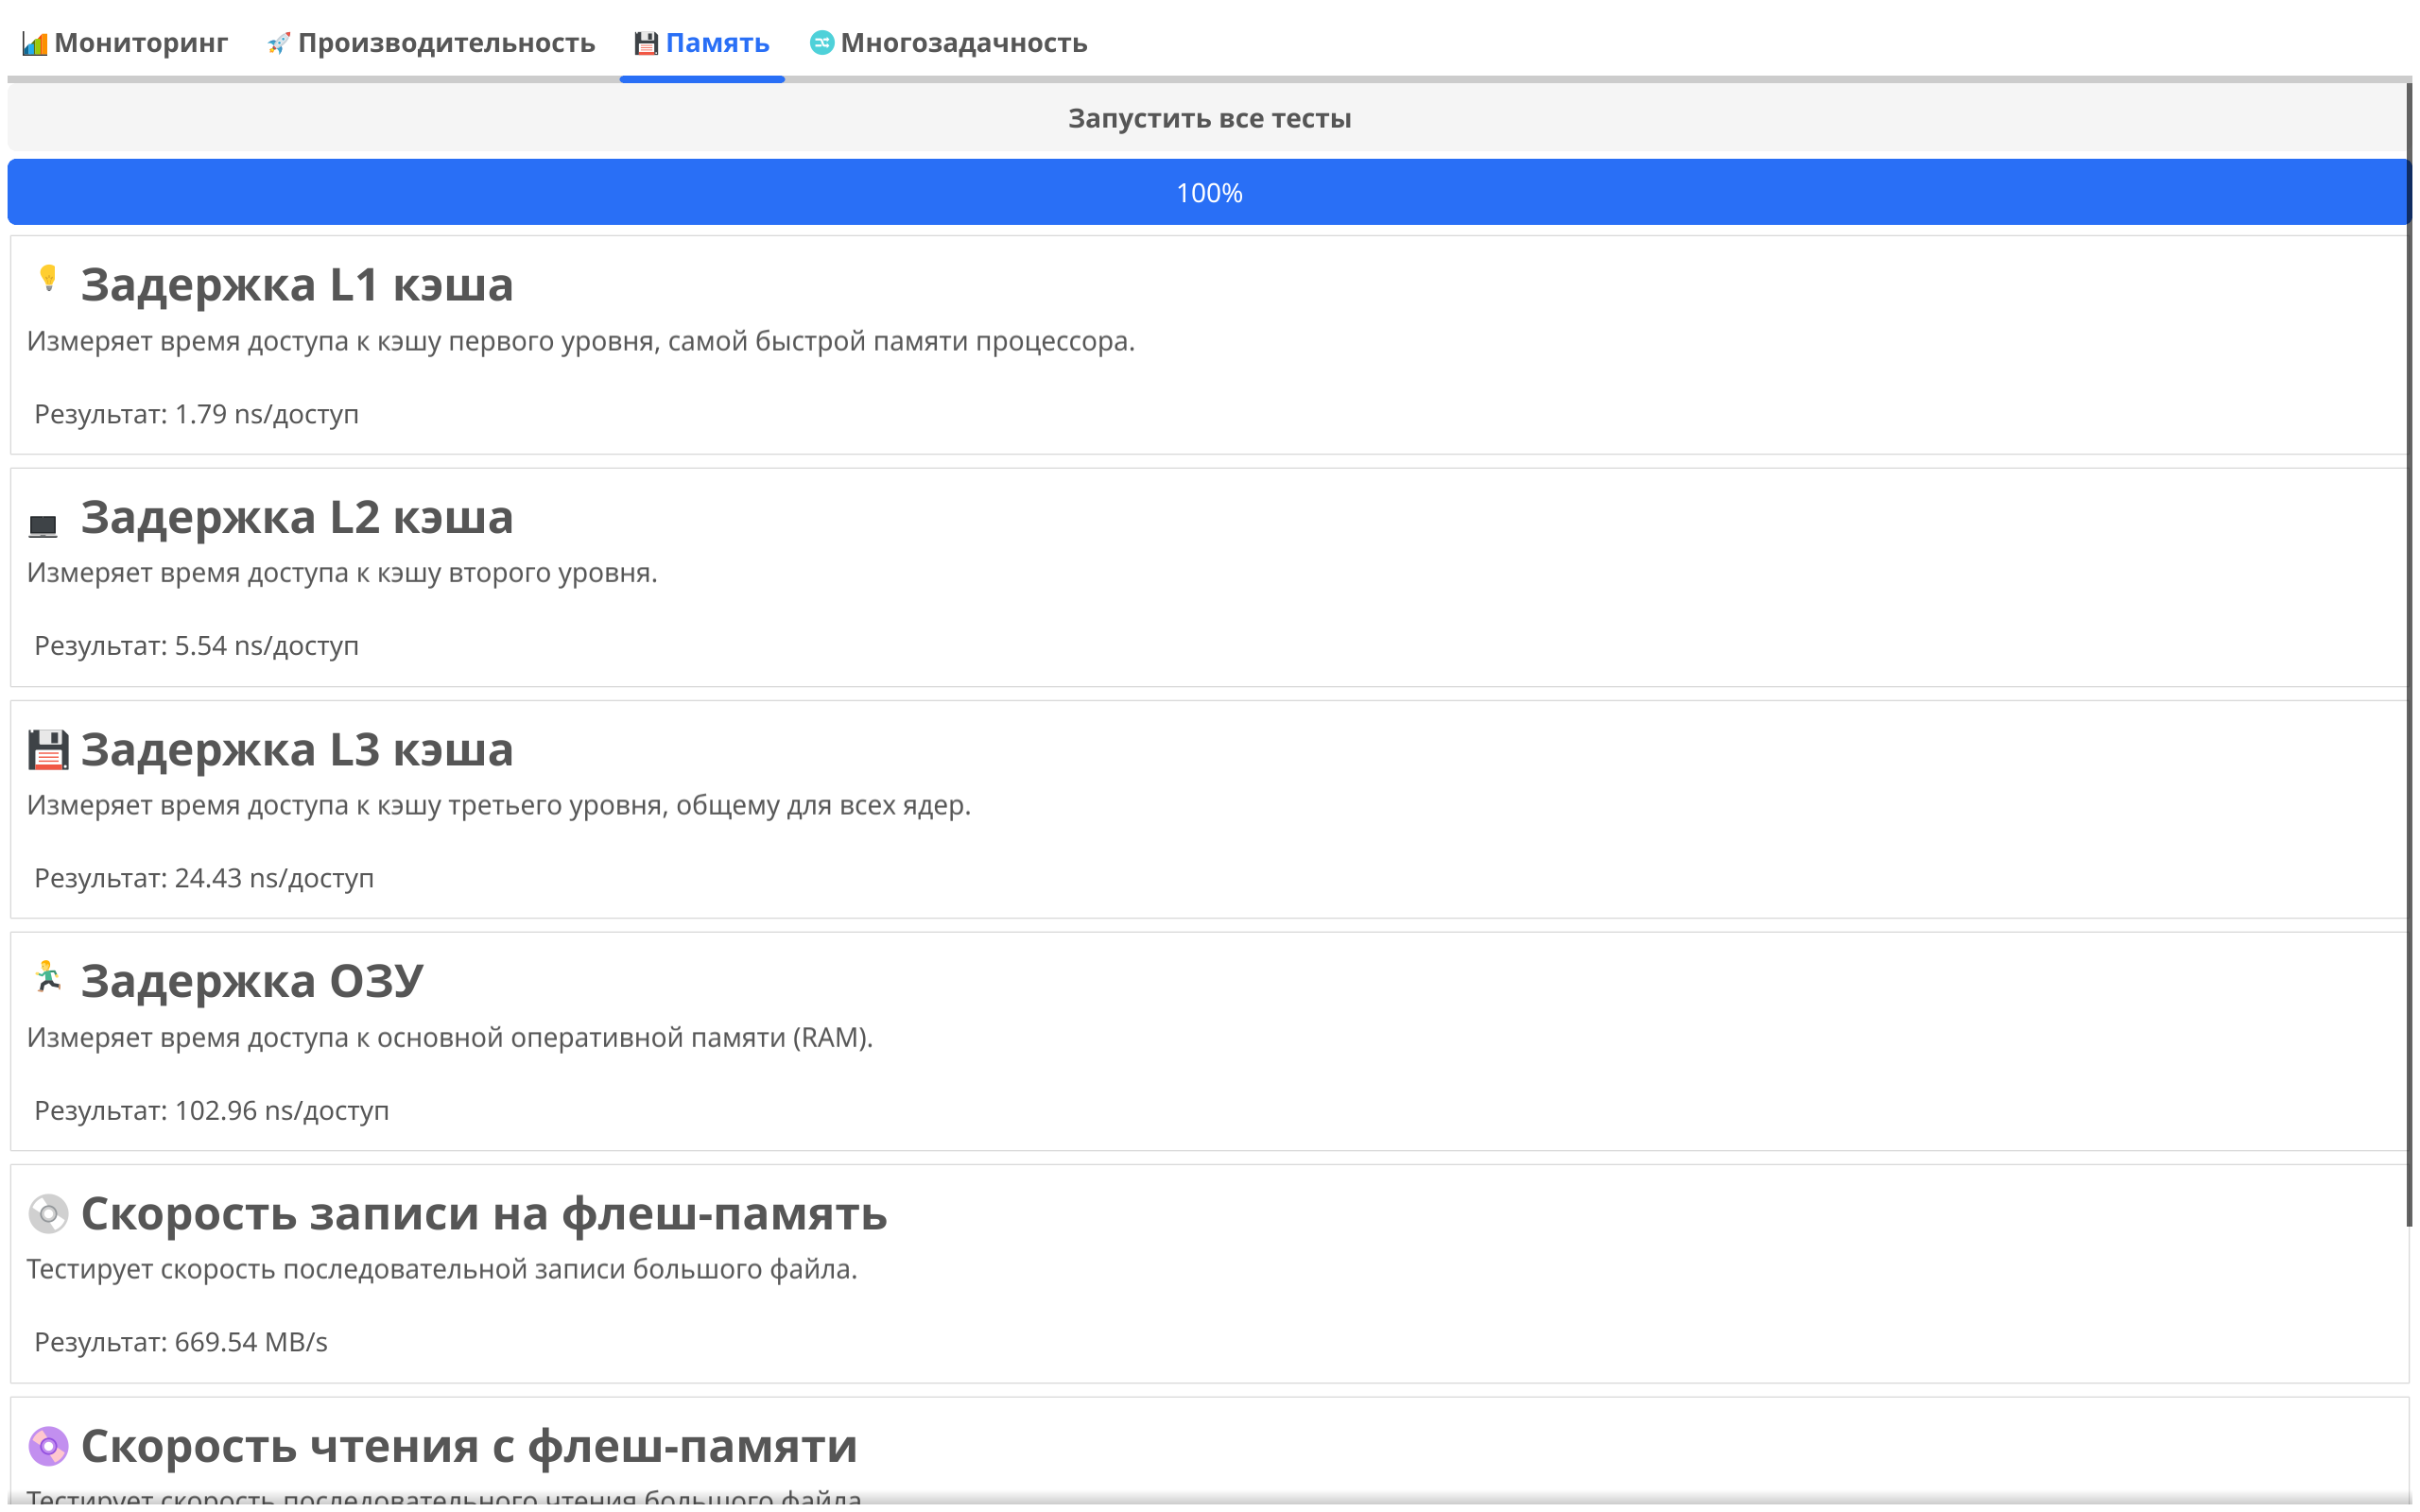
\includegraphics[width=0.92\textwidth]{memory_tests.png}
\caption{Пример панели тестов памяти и представления результатов}
\label{fig:memory_tests}
\end{figure}

Представленные скриншоты иллюстрируют, что экспериментальная работа с комплексом не сводится к консольному запуску отдельных утилит. Пользователь получает структурированный графический интерфейс, в котором мониторинг и бенчмарки сосуществуют в едином пространстве. Это особенно важно для экспериментов, ориентированных не только на получение числовых результатов, но и на интерпретацию условий их формирования.

\section{Контроль факторов, влияющих на корректность сравнения}

Сравнение двух вычислительных платформ всегда требует учёта факторов, которые затрудняют прямую интерпретацию чисел «в лоб». Даже если тестовая нагрузка одинакова на уровне исходного кода, реальное выполнение зависит от множества параметров: операционной системы, профиля энергопотребления, алгоритмов планировщика, поведения подсистемы памяти, драйверной модели и особенностей фоновых служб. Следовательно, любой сравнительный эксперимент должен сопровождаться фиксацией допущений и ограничений.

В рассматриваемой работе особое внимание уделяется следующим потенциальным источникам несопоставимости:
\begin{itemize}
    \item различие архитектур процессоров и наборов инструкций, что влияет на эффективность криптографических и арифметических операций;
    \item различие операционных систем, определяющее поведение планировщика, доступность телеметрии и характер фоновой активности;
    \item различие режимов энергосбережения и тепловых ограничений, особенно значимое для ноутбуков;
    \item возможное влияние кэширования, предвыборки и фоновых операций ввода-вывода на результаты коротких тестов;
    \item ограниченная воспроизводимость в условиях реального пользовательского окружения по сравнению с лабораторной стендовой средой.
\end{itemize}

Учёт перечисленных факторов не устраняет полностью вариативность измерений, но делает анализ более корректным. В частности, это позволяет отделять архитектурные различия платформ от случайных отклонений, связанных с моментным состоянием системы. Именно поэтому в рамках данного исследования результат рассматривается не как абсолютная и окончательная характеристика устройства, а как эмпирическая оценка его поведения в контролируемых, но реалистичных условиях эксплуатации.

\section{Формат представления результатов}

Для обеспечения сопоставимости итогов в работе используются единые правила представления и интерпретации результатов. Такой подход необходим, поскольку сравниваются не только разные платформы, но и разные классы нагрузок, для которых естественные единицы измерения принципиально различаются. Без предварительно заданных правил сравнение чисел разных типов было бы методически некорректным.

В качестве основных принципов принимаются следующие положения:
\begin{itemize}
    \item для показателей пропускной способности (МБ/с) сравниваются медианные значения;
    \item для латентности (нс) меньшие значения трактуются как более предпочтительные;
    \item для операций/с (например, RSA) большее значение соответствует более высокой производительности;
    \item коэффициент вариации рассматривается как индикатор устойчивости измерения.
\end{itemize}

Использование медианы в качестве базового сравниваемого показателя оправдано тем, что она менее чувствительна к единичным выбросам, чем среднее арифметическое. Это особенно важно в многозадачной среде, где даже один нехарактерный эпизод фоновой активности может заметно сместить среднее значение. Коэффициент вариации, в свою очередь, позволяет оценить, насколько надёжен наблюдаемый результат: высокая производительность при высоком разбросе не всегда предпочтительнее умеренной, но устойчивой производительности.

Для удобства дальнейшего анализа результаты целесообразно трактовать в двух плоскостях: количественной и качественной. Количественная плоскость отражает собственно числовое преимущество одной платформы над другой. Качественная плоскость показывает, как этот числовой результат соотносится с характером нагрузки и практическими сценариями применения. Такой двухуровневый подход делает экспериментальную часть более содержательной и приближает её к задачам реального системного анализа.

\section{Результаты и сравнение платформ}

Данный раздел предназначен для фиксации результатов экспериментального прогона комплекса на двух целевых платформах. Структурирование по категориям выбрано не случайно: оно соответствует логике самого программного комплекса и позволяет анализировать поведение систем не в виде общего «рейтинга», а по отдельным профилям нагрузки. Такой подход методически предпочтителен, поскольку одна и та же платформа может демонстрировать сильные стороны в одном классе задач и уступать в другом.

Таблицы ниже представляют форму документирования результатов, пригодную для последующего заполнения фактическими измеренными значениями. Важно подчеркнуть, что сами таблицы являются не просто способом визуального оформления, а частью методики: они задают единый формат фиксации результатов, минимизируют риск потери контекста и упрощают аналитическое сравнение после завершения серий прогонов.

\subsection{Процессорные тесты}

Процессорные тесты предназначены для оценки вычислительной мощности платформ, характера масштабирования по потокам и устойчивости поведения при нагрузках, чувствительных к структуре кода. В данной категории особенно важно учитывать не только итоговое значение, но и форму распределения нагрузки по ядрам, а также влияние архитектурных особенностей процессора, включая число производительных и энергоэффективных ядер, особенности кэш-подсистемы и динамическое изменение частот.

При анализе результатов CPU-бенчмарков необходимо обращать внимание на несколько аспектов. Во-первых, следует оценивать абсолютный уровень производительности, выраженный в прикладной единице измерения. Во-вторых, необходимо сопоставлять его со стабильностью результата: высокий разброс может свидетельствовать о сильном влиянии фоновой активности или о неустойчивом частотном режиме. В-третьих, полезно анализировать показания мониторинга в момент теста: равномерная загрузка ядер обычно соответствует корректному распараллеливанию, тогда как выраженная асимметрия может указывать на ограничения со стороны планировщика, синхронизации или архитектуры самой нагрузки.

\begin{table}[!htbp]
\centering
\caption{Сравнение процессорных тестов}
\label{tab:cpu_compare}
\begin{tabular}{|l|c|c|c|}
\hline
\textbf{Тест} & \textbf{Ед.} & \textbf{MacBook Air M2} & \textbf{Ryzen 5 4600H} \\
\hline
 &  &  &  \\
\hline
\end{tabular}
\end{table}

\noindent После заполнения таблицы интерпретация должна строиться не только на сравнении отдельных строк, но и на анализе общей картины. Если одна платформа демонстрирует преимущество в задачах с высокой долей ветвлений, но уступает в параллельных сценариях, это может указывать на различие в микроархитектурных приоритетах. Если же различия невелики, но коэффициент вариации заметно различается, практический вывод может заключаться не столько в абсолютном превосходстве, сколько в большей предсказуемости поведения одной из систем.

\subsection{Тесты памяти}

Тесты памяти направлены на исследование двух взаимосвязанных, но не тождественных характеристик: пропускной способности и латентности доступа. Эта категория особенно важна, поскольку в современных приложениях ограничение по памяти нередко проявляется скрыто и может ошибочно восприниматься как недостаток процессорной мощности. Сравнение платформ по параметрам памяти позволяет выявить, насколько эффективно каждая из них работает с большими потоками данных и насколько чувствительна к нерегулярным обращениям.

При интерпретации результатов памяти необходимо учитывать прикладной профиль задач. Высокая пропускная способность благоприятна для потоковой обработки, мультимедиа, некоторых научных и матричных вычислений. Низкая латентность особенно важна для сценариев, включающих сложные структуры данных, графы, базы данных, компиляторы и иные нагрузки с большим числом случайных обращений. Поэтому итоговый вывод по данной категории должен учитывать, какая именно характеристика памяти является более значимой для предполагаемого класса задач.

\begin{table}[!htbp]
\centering
\caption{Сравнение тестов памяти}
\label{tab:mem_compare}
\begin{tabular}{|l|c|c|c|}
\hline
\textbf{Тест} & \textbf{Ед.} & \textbf{MacBook Air M2} & \textbf{Ryzen 5 4600H} \\
\hline
 &  &  &  \\
\hline
\end{tabular}
\end{table}

\noindent При дальнейшем анализе желательно отдельно обсуждать ситуации, когда одна из платформ выигрывает по пропускной способности, а другая --- по латентности. Подобный результат не является противоречием; напротив, он отражает различие в архитектурных приоритетах и может иметь существенные прикладные последствия. Именно поэтому в рамках системного анализа память должна рассматриваться не как «один ресурс», а как совокупность характеристик доступа к данным.

\subsection{Математические тесты}

Математические тесты занимают промежуточное положение между «чисто процессорными» и более специализированными сценариями. С одной стороны, они в значительной степени зависят от общей арифметической мощности процессора и эффективности компиляции. С другой стороны, они могут демонстрировать чувствительность к организации циклов, локальности данных и особенностям работы с числами с плавающей точкой или целочисленной арифметикой.

В прикладном отношении данная категория важна для оценки пригодности платформы к задачам моделирования, аналитики, статистической обработки и инженерных вычислений. Если в рамках эксперимента наблюдается преимущество одной платформы в математических тестах, это может быть следствием как более высокой вычислительной плотности, так и лучшей адаптации микроархитектуры к соответствующему типу операций. В то же время стабильность результатов здесь не менее важна, чем абсолютные значения, поскольку математические сценарии нередко используются в длинных вычислительных цепочках, где предсказуемость времени исполнения имеет практическое значение.

\begin{table}[!htbp]
\centering
\caption{Сравнение математических тестов}
\label{tab:math_compare}
\begin{tabular}{|l|c|c|c|}
\hline
\textbf{Тест} & \textbf{Ед.} & \textbf{MacBook Air M2} & \textbf{Ryzen 5 4600H} \\
\hline
 &  &  &  \\
\hline
\end{tabular}
\end{table}

\noindent После заполнения данной таблицы интерпретация должна учитывать, насколько обнаруженные различия устойчивы между независимыми прогонами и коррелируют ли они с результатами общих CPU-бенчмарков. Если математические тесты повторяют картину процессорной категории, это усиливает уверенность в выводах. Если же наблюдается иная картина, это может быть поводом для более тонкого анализа архитектурных особенностей платформы.

\subsection{Криптографические тесты}

Криптографические тесты позволяют оценить поведение платформ в задачах, связанных с защитой информации, обработкой конфиденциальных данных и поддержкой защищённых коммуникаций. В отличие от общих CPU-бенчмарков, здесь результаты особенно чувствительны к наличию специализированных инструкций ускорения, качеству реализации библиотек и различию между алгоритмами симметричного, асимметричного и хеш-функционального типов.

Для симметричных алгоритмов ключевой характеристикой обычно является пропускная способность, определяющая потенциальную скорость обработки больших потоков данных. Для асимметричных алгоритмов важнее число операций в секунду, поскольку такие алгоритмы чаще используются в сравнительно коротких, но вычислительно дорогих операциях установления доверия, генерации подписей и проверки ключевого материала. Для хеширования существенна скорость обработки больших массивов данных, напрямую связанная с задачами контроля целостности, индексирования и построения цифровых отпечатков.

\begin{table}[!htbp]
\centering
\caption{Сравнение криптографических тестов}
\label{tab:crypto_compare}
\begin{tabular}{|l|c|c|c|}
\hline
\textbf{Алгоритм} & \textbf{Ед.} & \textbf{MacBook Air M2} & \textbf{Ryzen 5 4600H} \\
\hline
 &  &  &  \\
\hline
\end{tabular}
\end{table}

\noindent После получения фактических значений интерпретация этой таблицы должна учитывать, что «лучшая» платформа может различаться в зависимости от конкретного алгоритма. Преимущество в симметричном шифровании не гарантирует преимущества в асимметрических операциях, и наоборот. Именно поэтому криптографическая категория особенно показательна для демонстрации того, что универсального однозначного лидера по всем видам вычислительной нагрузки может не существовать.

\section{Выводы по экспериментальной части}

По итогам экспериментов должны быть сформулированы выводы о сравнительной производительности платформ в разрезе категорий нагрузок, а также о стабильности результатов, выдаваемых комплексом. При этом итоговая оценка не должна сводиться к упрощённому утверждению о том, что одна система «лучше» другой по всем параметрам. Гораздо более корректным является профильный вывод: одна платформа может оказаться предпочтительной для криптографических операций, другая --- для части вычислительных или память-зависимых задач, третьи особенности могут проявляться в стабильности и предсказуемости результата.

Не менее важным выводом экспериментальной части является подтверждение того, что разработанный комплекс позволяет анализировать платформу не в отрыве от контекста, а в связи с текущим состоянием системы. Именно наличие мониторинговой телеметрии, списка активных процессов, распределения нагрузки по ядрам и статистических характеристик измерения делает итоговые числа более содержательными и пригодными для инженерной интерпретации.

Отдельно должны фиксироваться ограничения сравнения: различие операционных систем, различие механизмов энергосбережения, особенности микроархитектуры, доступность аппаратных ускорителей, а также невозможность полного устранения внешних факторов в условиях пользовательской среды. Признание этих ограничений не ослабляет научную ценность эксперимента, а, напротив, делает анализ более корректным и методически добросовестным.

Таким образом, экспериментальная часть выступает логическим завершением всей работы: она демонстрирует, что разработанный программный комплекс способен выполнять не только функции визуализации и запуска тестов, но и служить инструментом получения воспроизводимых и интерпретируемых данных о вычислительных возможностях современных микропроцессорных систем.
